\section{Learning sparse seed regions from reduction time}
\label{sec:seed-geometry}
The batch study leaves little additional saving among its predefined partitions. We therefore change the equations available to Kira more directly. A learned boundary selects individual seeds around the requested numerator powers before equation generation. Kira then applies its usual IBP operators to those seeds. This follows the motivation of sparse target-dependent seeding~\cite{TubeSeeding2026}, while the boundary parameters in this study are fitted through complete reductions with symbolic dimension.

\subsection{The seed model and its training data}
The model describes a surrounding region around each target's numerator-power box. Its width can depend on the seed rank and on how many physical propagators are absent from its sector. It also controls the largest seed rank in each sector. Appendix~\ref{app:seed-geometry} defines these boundaries, derives the distance used by the model, and gives a counting example that explains why a narrow region can avoid many seeds at higher numerator rank.

We first fit the boundary parameters through evolutionary search. Each proposal runs Kira and receives a score from the measured time needed to reach the prescribed masters and pass an exact coefficient check. The score includes unsuccessful attempts and native recovery. Thus the labels describe completed calculations rather than membership in a previously selected equation set. Three training requests per graph start this search; separate validation selects the first fitted boundary. An independent planar-box comparison then tests that boundary on eight new kinematic requests.

The second stage adds twelve training requests per graph and fits models that predict the cost of different seed boundaries. These requests contain single-direction and distributed numerators of ranks two, three, and four. The candidate boundaries include those found by the first search, independent changes to the rank allowance, fixed surrounding widths, and unfiltered Kira. Trees and forests predict the log complete-time ratio of each candidate~\cite{CART1984,Breiman2001Forest,Geurts2006ExtraTrees}. Ten validation requests per graph select the model, its decision margin, and a fixed sparse control. The predictor is enabled only when validation gives at least three percent less recorded cost than that fixed control. When validation disables prediction, the deployed policy uses the selected fixed boundary. Table~\ref{tab:seed-geometry-models} gives the selected models. The independent timing tests include the cost of loading and applying them.

\begin{table}[!htbp]\centering\small
\caption{Cost predictors selected before the reserved comparisons. Each graph also has a separately selected fixed sparse control.}
\label{tab:seed-geometry-models}
\begin{tabular}{@{}llll@{}}\toprule
Graph & Predictor (depth) & Training requests & Deployment\\\midrule
Planar box & Tree (2) & 12 & Fixed boundary retained\\
Nonplanar box & Extra trees (2) & 12 & Enabled\\
\bottomrule\end{tabular}\end{table}

Validation enables request-dependent cost prediction for the nonplanar box. Other graph choices use their fixed sparse boundary.

\subsection{Independent reductions and controls}
The first evolved planar-box boundary gives 22.3\% less time, with a paired-repetition ratio interval of $[0.751, 0.813]$ relative to tuned native Kira. Relative to the fixed surrounding-width control, it gives 6.5\% less time, with a paired-repetition ratio interval of $[0.899, 0.980]$. This comparison contains 168 timed reductions, and all successful outputs pass exact checks. The boundary remains fixed throughout this test.

\begin{table}[!htbp]\centering\small
\caption{First independent planar-box comparison. Times are sums of per-request medians over eight requests, with seven repetitions per method. The learned boundary is fitted before this comparison.}
\label{tab:seed-geometry-initial}
\begin{tabular}{@{}lr@{}}\toprule
Method & Complete time (s)\\\midrule
Tuned native Kira & 37.893\\
Fixed surrounding width & 31.465\\
Evolved seed boundary & 29.424\\
\bottomrule\end{tabular}\end{table}

The second comparison uses 20 matched requests from the planar and nonplanar two-loop boxes, with seven repetitions per method. All methods use the same Kira executable, exact preparation, master basis, and native row elimination. The native control disables every learned choice. The fixed sparse control uses one validation-selected boundary per graph, including boundaries discovered during training, and performs no request-dependent cost prediction. The previous application retains the earlier published batch and equation policies. These controls separate the effect of sparse seeding from the added benefit of predicting which boundary to use for a particular target.

The complete selected workflow gives 22.2\% less time, with a paired-repetition ratio interval of $[0.764, 0.792]$ relative to tuned native Kira and 22.6\% less time, with a paired-repetition ratio interval of $[0.762, 0.789]$ relative to the previous application. Relative to the fixed sparse control, it gives 3.6\% less time, with a paired-repetition ratio interval of $[0.946, 0.981]$. Table~\ref{tab:seed-geometry-times} reports the measured times for both graphs. The comparison contains 560 timed reductions and 5600 exact coefficient comparisons. Failed reference requests number 0, and failed timed reductions number 0; these remain in the evidence record.

\begin{table}[!htbp]\centering\small
\caption{Sum of per-request median complete times, in seconds. Native uses the tuned outer bounds with all ML disabled. Fixed uses one sparse boundary per graph. Selected uses the frozen deployment policy.}
\label{tab:seed-geometry-times}
\begin{tabular}{@{}lrrrrr@{}}\toprule
Graph & Requests & Native & Previous & Fixed & Selected\\\midrule
Planar box & 10 & 20.986 & 21.072 & 15.742 & 15.802\\
Nonplanar box & 10 & 54.857 & 55.100 & 45.462 & 43.169\\
All matched & 20 & 75.843 & 76.172 & 61.203 & 58.972\\
\bottomrule\end{tabular}\end{table}

\begin{figure}[!htbp]\centering
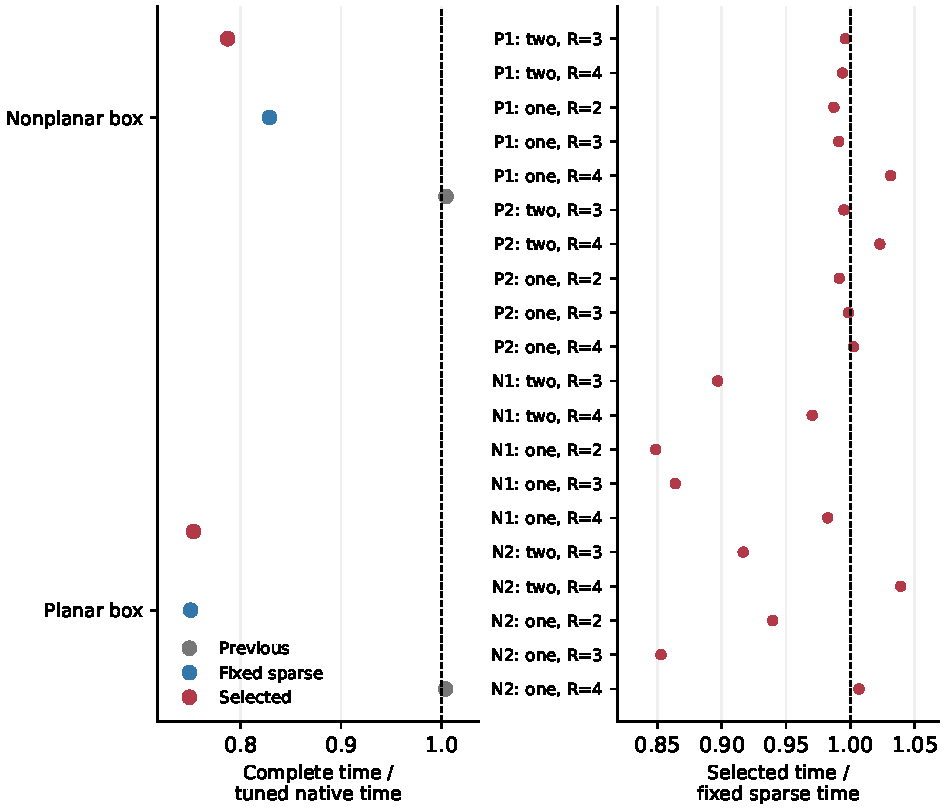
\includegraphics[width=\linewidth]{paper_figures/seed_geometry_times.pdf}
\caption{Left: complete-time ratios to tuned native Kira, summed within each graph. Right: the selected-to-fixed-sparse ratio for each reserved request. Labels P and N identify the planar and nonplanar graphs; 1 and 2 identify the two reserved kinematic profiles. Each label gives the number of powered numerator directions and the rank $R$. The dashed lines mark equal time. Values below one indicate a saving. The right panel shows the measured difference from using the fixed sparse rule.}
\label{fig:seed-geometry-times}
\end{figure}
\FloatBarrier

A separate application check starts a fresh process for each request and supplies only the physical definition, target indices, and master basis. It includes imports, model loading, input and output, process exit, and a subsequent exact check. It completes 48 runs over 4 matched requests. Its selected total is 15.774 seconds, compared with 27.897 seconds for native choices and 16.187 seconds for the fixed sparse control. These requests are a predefined subset of the reserved test, so they check application overhead without adding graph coverage.

The complete integrated application also passes 24 fresh-process checks. These use two of the reserved two-loop requests, one previously tested four-loop native request, and an eight-loop massless banana request. For the two-loop requests, the summed median complete time is 8.091 seconds, compared with 17.088 seconds for the preceding complete application. The other inputs check that the existing native and analytic methods remain available and exact. They do not extend the sparse model's fitted domain.

These results concern numerator ranks two through four, unit positive physical powers, rational kinematic values, symbolic dimension, and supplied bases in two known two-loop structures. The reported production times exclude offline training and construction of the independent reference basis. Some index patterns recur between training and testing. Development probes at other loop orders do not extend the fitted model's validated domain. The application retains its earlier exact methods and native fallback outside this domain. The comparison establishes the measured effects of the new seed policy; it does not establish a universal speedup or a globally optimal reduction path.
